In addition to probing BSM theories, taus offer a 
good laboratory for EW precision studies and for many observables (including $|V_{us}|$, $\alpha_s(m_\tau)$ and low-energy QCD quantities)~\cite{LusianiESPP19}.

\noindent
{\bf Lepton universality tests with taus:}
these are 
powerful probes to constrain new physics models (especially those 
designed to explain LFUV anomalies).
The most precise tests rely on measurements of the tau mass,
lifetime and leptonic branching ratios, respectively 
best measured by BES III, Belle and ALEPH 
with world-average uncertainties of 0.007\%, 0.172\% and 0.178\%~\cite{Tanabashi:2018oca}.
In the {\bf short- and mid-term}, these can be improved 
by exploiting high luminosity $e^+ e^-$ colliders
like Belle II~\cite{Abe:2010gxa,Kou:2018nap} and the SCT factories. In the {\bf long-term}, 
the proposed high energy $e^+ e^-$ colliders with high
luminosity runs at the $Z$ peak (\FCCee~\cite{Blondel:2019yqr}, 
\CEPC~\cite{CEPC_INPUT}, possibly \ILC~\cite{Baer:2013cma,Fujii:2017vwa}) also offer opportunities for tests of tau lepton universality. 

{\bf Tau LFV searches:} In the {\bf short-term}, 
Belle II has a reach of
order $10^{-9}$ for $\tau \to \mu \gamma$  and 
$10^{-10}$ for $\tau \to 3 \ell$~\cite{Kou:2018nap}, corresponding to a factor 10-50 improvement. This is illustrated in Fig.~\ref{fig:NPscales} (blue), for the reach in new physics scale. 
Belle II can also search for the rare decay $\tau \to \rho \gamma$ with a projected sensitivity of $2\times 10^{-10}$ (at 50~ab$^{-1}$)~\cite{Kou:2018nap}. 
In the {\bf mid-term},  
the two SCT projects~\cite{Bondar:2013cja,Novosibirsk_SCT_input,Luo:2018njj,Peng:2018} offer favourable conditions for a competitive reach on $\tau \to \mu \gamma$. 
TauFV (planned at the Beam-Dump Facility of the
SPS, upstream of SHiP)~\cite{TauFV_input}
is a fixed-target experiment designed to search for LFV in tau decays, 
benefiting from technological developments being
pursued for the \HLLHC experiments and future hadron colliders.
TauFV's sensitivity to the $\tau \to 3 \mu$ decay
may improve that of Belle II.
In the {\bf longer term}, runs at the $Z$ pole of \FCCee (\CEPC)
can deliver 
$15\times 10^{10}$ ($3 \times 10^{10}$) $\tau$ pairs~\cite{Blondel:2019yqr, CEPC_INPUT}; 
improvements of an
order of magnitude with respect to Belle II may thus be possible. 


{\bf Precision tau measurements:}
In the {\bf short-term}, Belle II has the potential for improvements,
at the price of considerable work on the limiting systematics. 
In the {\bf mid-term}, the programmes of the STC factories include precision
measurements of low multiplicity tau branching ratios, and
offer by far the best prospects regarding tau mass measurements~\cite{Bondar:2013cja,Novosibirsk_SCT_input,Luo:2018njj,Peng:2018}: 
$\Delta m_\tau = \pm 0.012$~MeV, due to a reduction of systematic errors
(for Belle II, 
$\Delta m_\tau = 
\pm 0.10 - 0.15$~MeV~\cite{Kou:2018nap}). 
In the {\bf long term}, future $e^+ e^-$ colliders operating at the $Z^0$
pole offer the best conditions for significant advances. 
For BR($\tau \to \ell \bar \nu\nu$), 
 both \FCCee and \CEPC can
reach a precision of 0.02\%~\cite{Blondel:2019yqr,CEPC_INPUT}. For the tau lifetime, 
\FCCee aims at a precision  
$\Delta \tau_\tau \sim 0.01\%$ 
(to be compared with 0.026\% at Belle II). For tau mass measurements, \FCCee is less performant than the other possible projects: 
by calibrating on $m_{D^+}$, it aims at 
$\Delta m_\tau = 0.07$~MeV.


A  summary of the above sensitivity goals and prospects concerning $\tau \to 3\mu$ decays and $m_\tau$ can be found in Fig.~\ref{fig:Lusiani_prospects}.

\begin{figure}
\centering
\hspace*{-3mm}
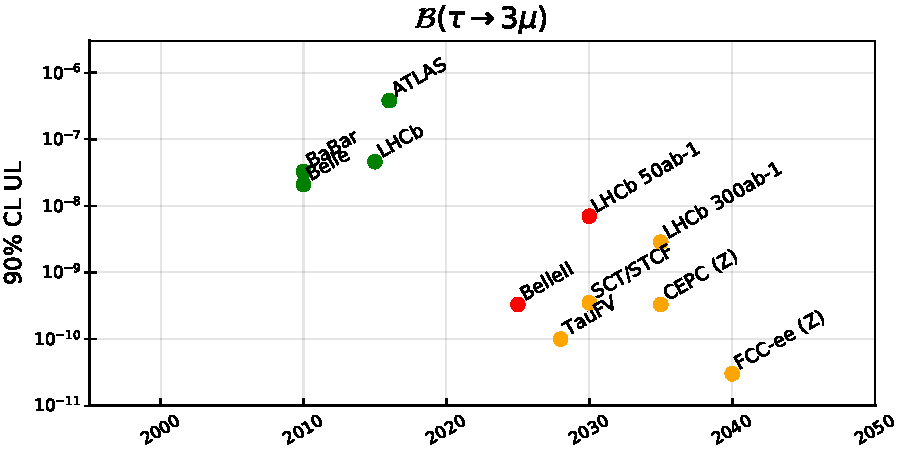
\includegraphics[width=0.75\textwidth]{\main/Flavour/figs/ul90cl-tau-3mu-esg-may19} 
\vspace*{3mm}\\
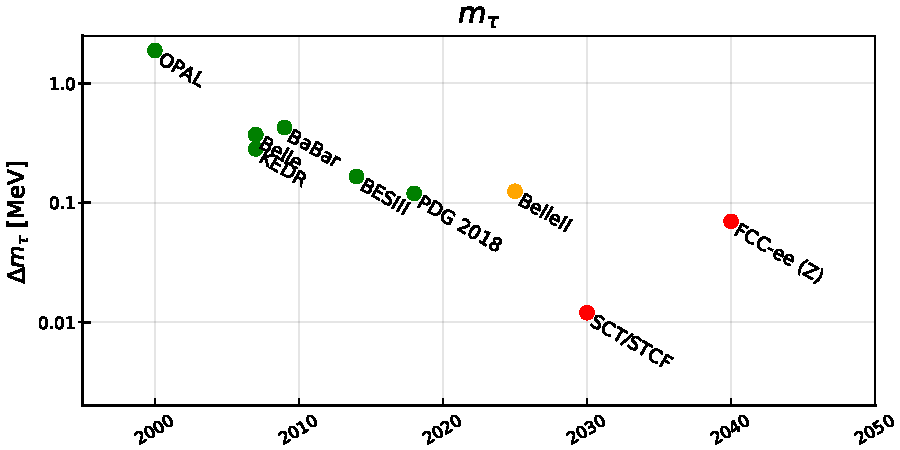
\includegraphics[width=0.75\textwidth]{\main/Flavour/figs/unc-tau-mass-esg-may19} 
\caption{Expected sensitivity and projected precision of  present and future experiments for $\tau \to 3\mu$ decays and $m_\tau$~\cite{LusianiESPP19}.
Green denotes current measurements, red  points correspond to estimates of future experimental sensitivities based on dedicated studies (relying on extrapolation from past established performances) while orange corresponds to estimates of experimental sensitivities including novel features (for which extrapolation from past experience is more difficult). }\label{fig:Lusiani_prospects} 
\end{figure}
